\model{Die objects}
\label{CS1/class-die}

\begin{quote}
\hfill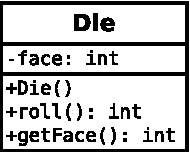
\includegraphics{CS1/Die.pdf}
\vspace*{-84pt}

\begin{javalst}
/**
 * Simulates a Die object.
 */
public class Die {
    
    private int face;
    
    /**
     * Constructs a new die with a random face value.
     */
    public Die() {
        face = 1;
    }
    
    /**
     * Gets the current face value of the die.
     *
     * @return current face value of the die
     */
    public int getFace() {
        return face;
    }
    
    /**
     * Simulates the roll of the die.
     *
     * @return new face value of the die
     */
    public int roll() {
        face = (int) (Math.random() * 6) + 1;
        return face;
    }
    
}
\end{javalst}

\vspace*{-128pt}
% https://commons.wikimedia.org/wiki/File:2-Dice-Icon.svg
\hfill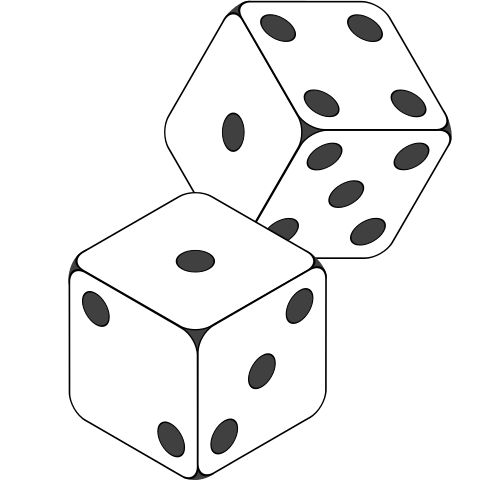
\includegraphics[width=2in]{CS1/dice.png}
\end{quote}


\quest{10 min}


\Q What are the attributes of \java{Die}? What are the methods?

\begin{answer}
The only attribute is \java{face}. The methods are \java{Die}, \java{roll}, and \java{getFace}.
\end{answer}


\Q In the class diagram, what do the \java{-} and \java{+} symbols represent? What does the \java{:} represent?

\begin{answer}
Plus means {\tt public}, minus means {\tt private}, and colon refers to the data type.
\end{answer}


\Q Write a statement that \emph{declares} a \java{Die} variable named \java{lucky}.

\begin{answer}
\tt Die lucky;
\end{answer}


\Q Each \emph{instance} of a class (in memory) is called an object. Write a statement that \emph{instantiates} a \java{new} \java{Die} object and assigns it to \java{lucky}.

\begin{answer}
\tt lucky = new Die();
\end{answer}


\Q When you instantiate an object, you invoke a \emph{constructor}.
This method has no return type and has the same name as the class itself. What does the \java{Die} constructor do?

\begin{answer}
It ``rolls'' the die by calling the \java{roll} method.
\end{answer}


\Q Notice how the \java{roll} method refers to \java{face}, yet that variable is not declared in the method. What does the \java{roll} method change, in terms of the \java{Die} object?

\begin{answer}
It updates the value of the \java{face} attribute.
\end{answer}


\Q What is the purpose of the \java{getFace} method? Show how you would use it in a \java{main} method of another class.

\begin{answer}
It updates the value of the \java{face} attribute. In a {\tt main} method, you would do something like: {\tt System.out.println(lucky.getFace());}
\end{answer}
